\section{Lateral water impact 1x, with Ghost particles boundary condition}
\label{ss:example:lateral_water_1x_ghost}
%
\subsection{General}
%
This example solves the same case of the previous example described in the section
\ref{ss:example:lateral_water_1x_deleffe}, but changing the boundary condition from the De Leffe's
type to a ghost particles one, discussed on section \ref{sss:aquagpusph:boundaries:ghostparticles}.\rc
%
The objective of this example is to show how the ghost particles are used and to get a comparison on
the results obtained with each type of boundary condition.\rc
%
At the other hand, in the previous example the full process to generate a case has been documented, but
in this case we will cover only the differences with the previous example, using installed resources to run
it.\rc
%
The topics that will be covered in this example are:
%
\begin{enumerate}
	\item Configuration differences due to the boundary condition change.
	\item How to run and track a simulation installed on the system.
	\item Results comparison using either boundary integrals or ghost particles boundary conditions.
\end{enumerate}
%
In order to get a ready to run instance of this example, 2D version of \NAME package must be built, and examples
must be switched on at CMake configuration, as described in section \ref{sss:install:cmake}. You can find the
example either on the built package, at the subfolder ``examples'', and on the installed package, at\\
``\$\{CMAKE\_INSTALL\_PREFIX\}/\$\{CMAKE\_INSTALL\_DATADIR\}/examples'' (see section \ref{sss:install:cmake} to
learn more about this folder).\rc
%
Hereinafter we assume that ``\$\{CMAKE\_INSTALL\_PREFIX\}'' has been set as ``/usr'', and the example can be
found at ``/usr/share/aquagpusph/examples/LateralWater\_1x\_Ghost'' therefore.
%
\subsection{Case description}
%
You can find the case description in the section \ref{sss:example:lateral_water_1x_deleffe:caseDescription},
where the same case has been described.
%
\subsection{Settings changes required to modify the boundary condition}
%
During the section \ref{sss:example:lateral_water_1x_deleffe:BC} how to set a De Leffe's type of boundary
condition has been described. In this case this boundary condition must be deactivated, but we can use the
area elements generated to set a ``ElasticBounce'' boundary condition, described in section
\ref{sss:aquagpusph:boundaries:elasticbounce}, in order to avoid the particles trespass the walls, so the option
``Boundary'' must be moved to ``ElasticBounce'':
%
\begin{verbatim}
<Option name="Boundary" value="ElasticBounce" />
\end{verbatim}
%
Ghost particles walls are set in a different way of the other boundary conditions, where a set of special
particles are used. To set ghost particles driven walls a file called ``\textbf{GhostParticles.xml}'' is
created with the following content:
%
\begin{verbatim}
<?xml version="1.0" ?>
<sphInput>
	<GhostParticles>
		<TangentUModel value="SSM" />
		<Wall>
			<Vertex x="-0.45" y="0.0" />
			<Vertex x="0.45" y="0.0" />
		</Wall>
		<Wall>
			<Vertex x="0.45" y="0.0" />
			<Vertex x="0.45" y="0.508" />
		</Wall>
		<Wall>
			<Vertex x="0.45" y="0.508" />
			<Vertex x="-0.45" y="0.508" />
		</Wall>
		<Wall>
			<Vertex x="-0.45" y="0.508" />
			<Vertex x="-0.45" y="0.0" />
		</Wall>
		<Wall>
			<Vertex x="-0.704" y="0.254" />
			<Vertex x="0.0" y="-0.45" />
		</Wall>
		<Wall>
			<Vertex x="0.0" y="-0.45" />
			<Vertex x="0.704" y="0.254" />
		</Wall>
		<Wall>
			<Vertex x="0.704" y="0.254" />
			<Vertex x="0.0" y="0.958" />
		</Wall>
		<Wall>
			<Vertex x="0.0" y="0.958" />
			<Vertex x="-0.704" y="0.254" />
		</Wall>
	</GhostParticles>
</sphInput>
\end{verbatim}
%
In this case symmetric tangential velocity model is imposed in order to simulate free-slip boundary
condition.\rc
%
Of course this file must be referenced into ``\textbf{Main.xml}'' file too.\rc
%
Since the ``ElasticBounce'' boundary condition has been retained, the spatial discretization still being valid.
%
\subsection{Running the example installed version}
\label{ss:example:lateral_water_1x_ghost:running}
%
In this example the installed version of the example will be directly executed. To do it, create a folder
to work, for instance, a folder called ``LateralWater\_1x\_Ghost'' in your home folder, and move into:
%
\begin{verbatim}
mkdir ~/LateralWater_1x_Ghost
cd ~/LateralWater_1x_Ghost
\end{verbatim}
%
The example provides a bash script that allows to easily run the case and plot the results during the
simulation. To run the simulation type:
%
\begin{verbatim}
/usr/share/aquagpusph/examples/LateralWater_1x_Ghost/run.sh --run
\end{verbatim}
%
This command will launch \NAME with the input file set and reassembly switched off, after cleaning previous
execution results. In this case the simulation can take more time due to this boundary condition can be really
less computational efficient.\rc
%
This case will turn unstable and stop running at simulation time of 4.57208 seconds, with a time step too low to
can continue working, so when this happens cancel the job pressing `\textbf{c}' key (allowing \NAME to close
properly the case).
%
\subsection{Post-process the simulation}
\label{ss:example:lateral_water_1x_ghost:postprocess}
%
The case post-process documented along the section \ref{ss:example:lateral_water_1x_deleffe:postprocess}
still being valid in this case, but for the plotting process we can use the provided script. In another
terminal we can start the plot process executing:
%
\begin{verbatim}
/usr/share/aquagpusph/examples/LateralWater_1x_Ghost/run.sh --plot
\end{verbatim}
%
Previous command copy the motion and pressures experimental registry into the execution folder, and launch
\textit{gnuplot}. In the figure \ref{fig:examples:lateral_water_1x_ghost:sensors} the pressure register
computed using Ghost particles and the experimental one are shown. Can be noticed that with the same
resolution and number of neighbours, this boundary condition returns really worst results than the shown
in the figure \ref{fig:examples:lateral_water_1x_deleffe:sensors}, corresponding to a De Leffe's type 
free-slip boundary condition.\rc
%
In the figure \ref{fig:examples:lateral_water_1x_ghost:paraviewanimation} the first impact visualization is
shown.
%
\begin{figure}[h!]
  \centering
  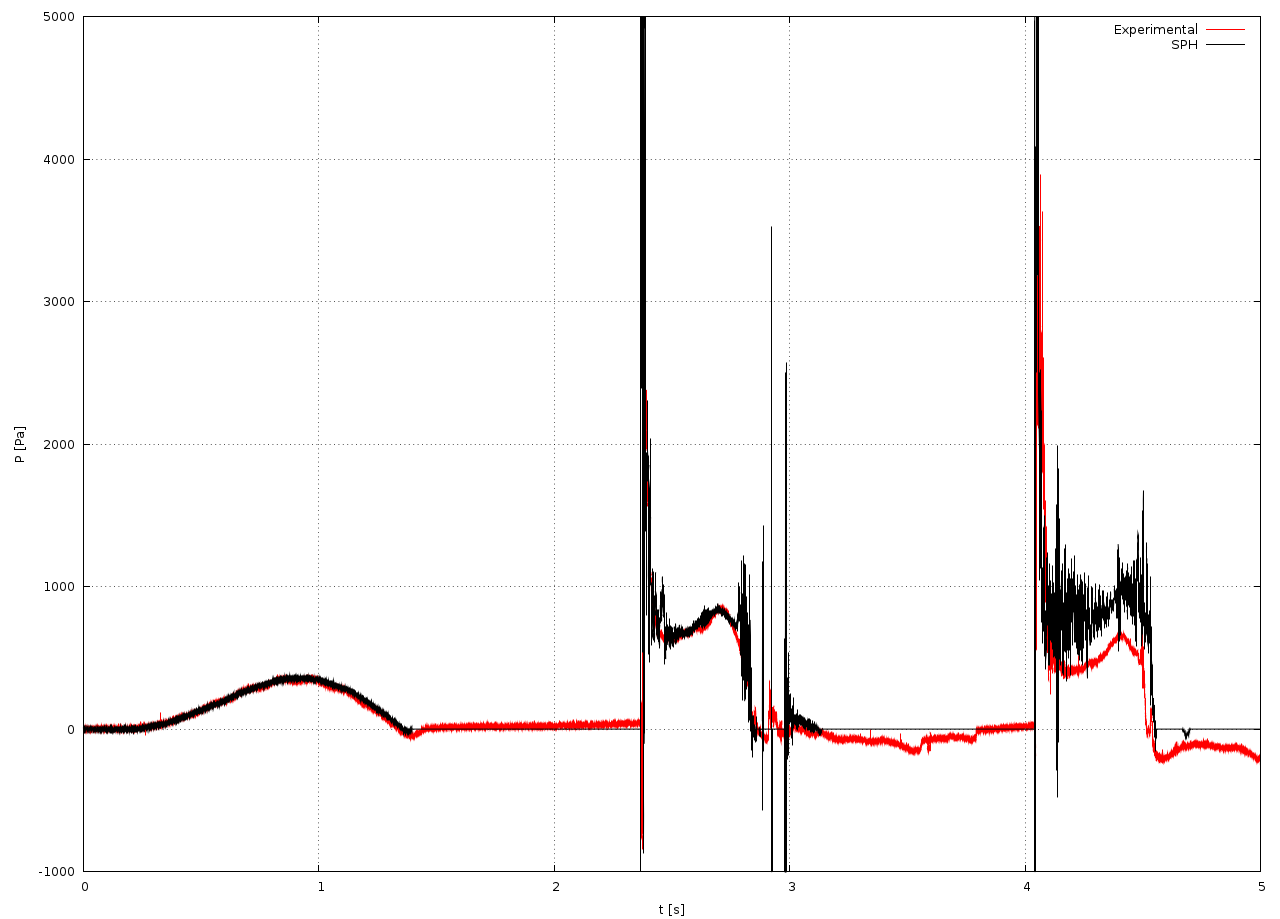
\includegraphics[width=0.7\textwidth]{lateral_water_1x_ghost/sensors_freeslip}
  \caption{Pressure register comparison between experimental and simulation data, using ghost particles and
  free-slip boundary condition (Tangent velocity SSM model)}
  \label{fig:examples:lateral_water_1x_ghost:sensors}
\end{figure}
%
\begin{figure}[ht!]
  \centering
  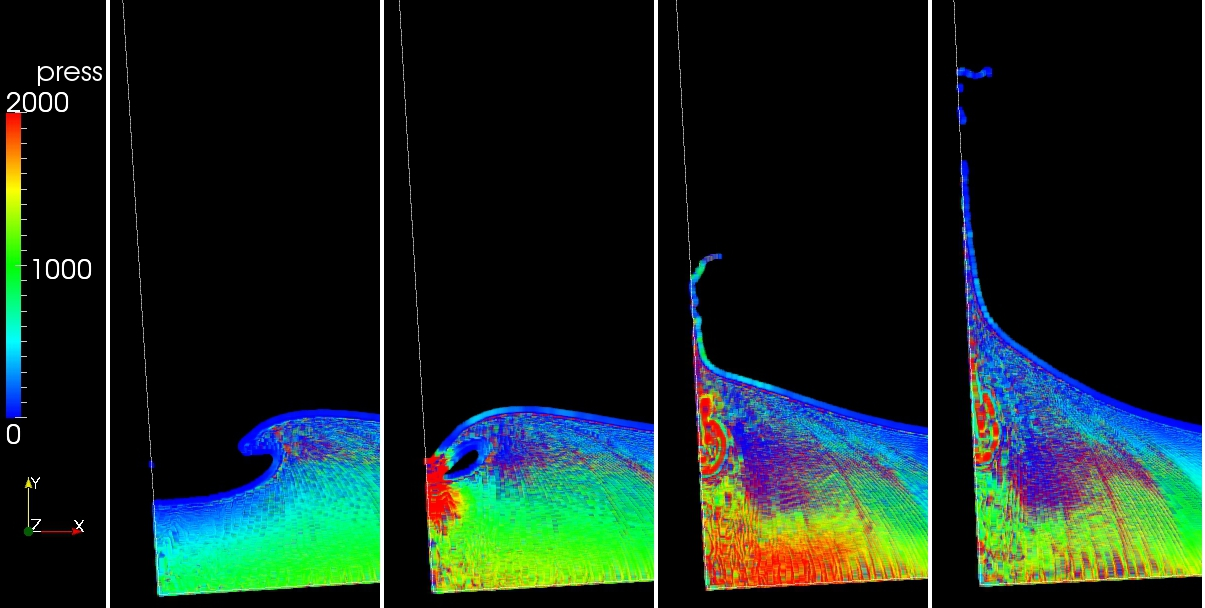
\includegraphics[width=0.7\textwidth]{lateral_water_1x_ghost/animation_freeslip}
  \caption{Animation of the example for the first impact, frames 70-73, using ghost particles and free-slip
  boundary condition}
  \label{fig:examples:lateral_water_1x_ghost:paraviewanimation}
\end{figure}
%
\subsection{Conclusions}
\label{ss:example:lateral_water_1x_deleffe:conclusions}
%
In this example two different boundary conditions has been test, the boundary integrals used in the previous
example, and the ghost particles documented along this one. Comparing figures
\ref{fig:examples:lateral_water_1x_deleffe:sensors} and \ref{fig:examples:lateral_water_1x_ghost:sensors},
corresponding to boundary integrals and ghost particles, you can see that the first one is able to reproduce
better the experimental wave impact pressure register at sensor 1.\rc
%
Also a SPH instability has been experienced in this case, causing the program crash due to a too small time step
for the used precision.\rc
%
In order to control the instability we can consider to set a no-slip boundary condition, that in the case of
ghost particles is set with the tangential velocity model, changing it from a symmetric model ``SSM'' to an
antisymmetric model ``ASM''.
%
\begin{verbatim}
<TangentUModel value="ASM" />
\end{verbatim}
%
But ``ASM'' model is inconsistent for almost general velocity fields when the Laplacian is computed, as
\ref{MaciaetalPTP} shown with polynomial velocity fields, so as $h \rightarrow 0$ the accelerations will blows up therefore, that in this case (where the resolution is fine enough) will accelerate the instability.\rc
%
In figure \ref{fig:examples:lateral_water_1x_ghost:sensors_noslip} the simulation pressure register computed until
$t \le 0.7328 s$, where the first instabilities can be appreciated much earlier than in the free-slip case.
%
\begin{figure}[h!]
  \centering
  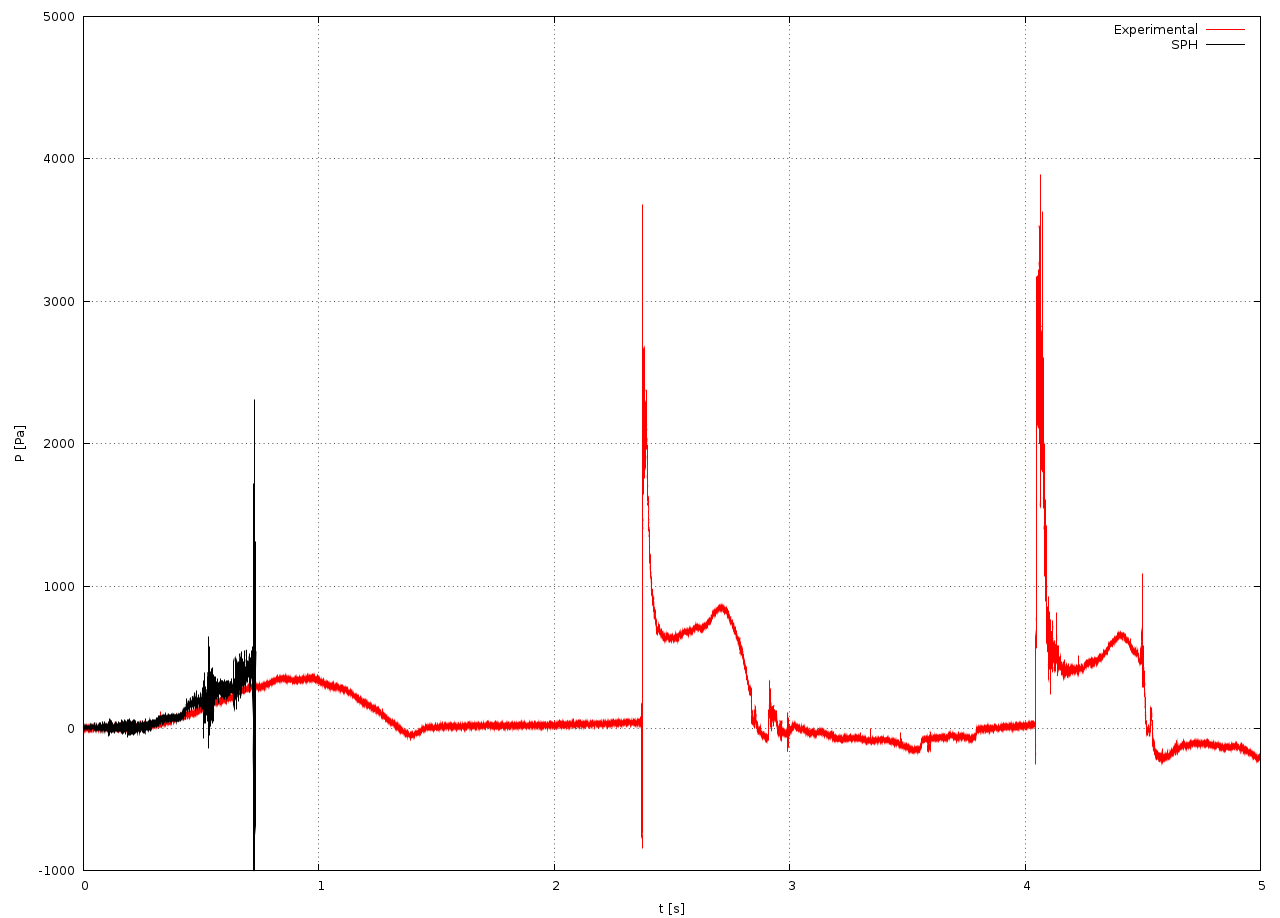
\includegraphics[width=0.7\textwidth]{lateral_water_1x_ghost/sensors_noslip}
  \caption{Pressure register comparison between experimental and simulation data, using ghost particles and
  no-slip boundary condition (Tangent velocity ASM model)}
  \label{fig:examples:lateral_water_1x_ghost:sensors_noslip}
\end{figure}
%
